%As mentioned in section \ref{sec:bg}, the built-in deadlock detector (if not disabled \cite{go-netDeadlock}) only detects global deadlocks where the main goroutine is blocked and ignores other goroutines' states. For instance, more than 70\% of blocking bugs (partial deadlocks and leaks) in GoKer \cite{yuan-gobench-cgo21} are not detectable by the built-in deadlock detector.
%
\subsection{Overview}
\label{sec:overview}
Figure \ref{fig:goat_workflow} displays the workflow of \goat to achieve objectives that introduced in section \ref{sec:intro} towards testing and debugging blocking bugs.
%
Given a program \textbf{P} (\ie, a set of Go source files with a \textit{main} function), \goat automatically instruments \textbf{P} and constructs static and dynamic models of execution for thorough testing and analysis.
%
\goat's work starts with parsing source files to identify and instrument the location of concurrency primitive usages in \textbf{P} (section \ref{sec:static_analysis}).
%
We inject \goat handlers around such locations to effectively perturb the blocking behavior of \textbf{P}.
%
\goat also constructs a fixed model from the concurrency usage to maintain coverage measurements during testing iterations (section \ref{sec:coverage}).
%
The instrumented \textbf{P} is then built and executed in the \goat runtime that supports execution concurrency tracing and schedule-space exploration (section \ref{sec:dynamic_analysis}).
%
Once the execution of \textbf{P} terminates (\eg, successfully exits , fails, times out), an ECT (execution concurrency trace) containing sequence of executed events is generated to get analyzed in offline (section \ref{sec:offline_analysis}).
%
If we detect a bug or the coverage reaches a threshold, \goat terminates the process and generates reports for the user (section \ref{sec:reports}). Otherwise, \goat continues the testing iteration until the termination condition met.
%
The remainder of this section describe the design and implementation of each component of \goat.

\subsection{Static Analysis}
\label{sec:static_analysis}
To gain insight into the behavior of P, \goat statically constructs a model from the usage of concurrency primitives and enables uniform analysis and update during testing iterations.
%
The model is a table of source locations (files and line numbers) that correspond to concurrency primitive actions (\eg, channel send or mutex unlock).
%
Such actions define the concurrent behavior (\ie, non-determinitstic blocking interaction between concurrent components) of P.
%
\goat inject random and bounded delays at these source locations to explore feasible scenarios and accelerate the exposure of rare bugs.
%
In section \ref{sec:covreq}, we describe the other advantage of concurrency usage model in defining concurrent coverage requirements and their dynamic measurements.
%

By traversing the \textit{abstract syntax tree} (AST) for each of source files in \textbf{P} using the Go AST package~\cite{go-package-ast}, \goat constructs the concurrency usage \textit{concurrency usages} (CU) model.
%
We also identify the main function during AST traversal to equip \textbf{P} with concurrency tracing mechanism.

\subsubsection{Concurrency Usage Identification}

We define \textit{concurrency usage} (CU) as a triple of $(f,l,k)$ where $f$ is the file name, $l$ is the line number and $k$ is the kind of concurrency primitive used in the code location.
Kind $k\in$ \texttt{Channel} $\cup$ \texttt{Sync} $\cup$ \texttt{Go} where:
\begin{itemize}
  \item \texttt{Channel} = \{\texttt{send}, \texttt{receive}, \texttt{close}\}
  \item \texttt{Sync} = \{\texttt{lock}, \texttt{unlock}, \texttt{wait}, \texttt{add}, \texttt{done}, \texttt{signal}, \texttt{broadcast}\}
  \item \texttt{Go} = \{\texttt{go}, \texttt{select}, \texttt{range}\}
\end{itemize}

The first column of table \ref{tab:moby_cov_table} shows the critical points extracted from program in listing \ref{listing:moby28462.minipage}.
%
\goat injects its handlers before CU points are the entry points to inject delay handlers of \goat to inject scheduler perturbation handlers before these points.

%

\subsection{Coverage Requirements}
\label{sec:covreq}
Based on our observations from execution of Go applications and bug kernels on the behavior of concurrency primitives, we define a set of coverage requirements (summarized in table \ref{tab:cov_req}):
%
\begin{itemize}
  \item \textbf{Req1 (Send/Recv):} \{\texttt{blocked}, \texttt{unblocking}, \texttt{NOP}\} -- Goroutine $G_1$ is either \textit{blocked} on a channel send (receive) if the receiver (sender) goroutine $G_2$ is not ready or \textit{unblocking} the waiting receiver (sender) goroutine $G_2$. A channel send or receive might also be neither blocked nor unblocking (NOP) for buffered channels.
  \item \textbf{Req2 (Select-Case):} \{\texttt{blocked}, \texttt{unblocking}, \texttt{NOP}\} $\times$ \{\texttt{case}$_i$\} -- cases of select statements are channel sends and recives (or default case for non-blocking selects). For all select statements that has no default case, we obtain the cases of each select statement at runtime and maintain an instance of Req1 per case.
  \item \textbf{Req3 (Lock):} \{\texttt{blocked}, \texttt{blocking}\} -- Goroutine $G_i$ is either \textit{blocked} when locking a mutex because another goroutine has locked the mutex or \textit{blocking} other goroutines from acquiring the mutex lock.
  \item \textbf{Req4 (Unblocking):} \{\texttt{unblocking}, \texttt{NOP}\} -- The goroutine that is performing channel close, mutex unlock, conditional variable signal and broadcast, waitGroup done and non-blocking select case (send or receive) has two kinds of behavior. They either \textit{unblock} one or more waiting goroutines or has no effect (NOP).
  \item \textbf{Req5-Go:} \{\texttt{NOP}\} -- We emit a NOP action for each goroutine creation to indicate that it is covered during testing.
\end{itemize}


These requirements are effective because with the help of \goat infrastructure, they satisfy the characteristics of an ``acceptable'' coverage metric:
\begin{itemize}
  \item A \textit{fixed concurrency model} from target application is statically obtained by identifying CU points.
  \item We can measure whether the requirement has been covered by analyzing the test ECT. By maintaining a global data structure during execution of all $t \in \mathcal{T}$, we can evaluate the coverability of proposed requirements
  \item Every uncovered requirement report something meaningful. For example, if a send is always performing as \textit{unblocking} and never as \textit{blocked}, which means that receiver of this send always performs receive before sender reaches its send statement. In other words, the receive action \textit{always happen-before} send action. Perhaps this pattern of communication is part of the program semantic and matches developer's expectations (e.g., a set of goroutines are listening on a channel to perform non-frequent requests). Otherwise, it reflects a bug or flaw in the program design.
  \item Since \goat is able to detect occured blocking bugs and also maintain a global coverage model during testing iterations, testing phase can terminate either by detection of a bug or reaching a coverage percentage threshold.
\end{itemize}


\subsection{Dynamic Analysis}
\label{sec:dynamic_analysis}
The primary cause of most real-world concurrent bugs is the misuse of concurrency features like channels, mutexes, and waitGroups (table \ref{tab:comparison}).
%
To gain insight into the behavior of concurrency features during execution, we equipped \goat with a tracing mechanism~\cite{ect-arxiv}, which is an extension to the Go built-in tracer package~\cite{go-cmd-trace}.
%
The tracing capability is compiled into all programs always through the runtime and is enabled on demand -- when tracing is disabled, it has minimal runtime overhead \cite{go-exec-tracer-doc}.
%
We chose the tracer package to enhance because it 1) is already compiled into the runtime, 2) adds minimal overhead, and 3) only lacks some pieces allowing the construction of an accurate concurrency model.
%
The concurrency tracing capability is added to the original Go runtime through a one-time patch~\cite{ect-patch}.

\subsubsection{Execution Concurrency Tracing (ECT)}
\textit{Execution concurrency trace} (ECT) is a totally ordered \textit{sequence} of events in which the order is approximated through a central clock with nanosecond precision.
%
ECT also contains the call-stack for each event, enabling a direct mapping of events to source-line numbers.
%
The alphabet of ECT is total of 63 events -- 49 from original tracer package \cite{goParserSource}, categorized and summarized in table \ref{tab:events} and 14 additional events that we added to capture concurrency usage events:
%
\begin{itemize}
    \item \textbf{Channel:} For each channel operation (make, send, receive, close), ECT includes an event with a unique id assigned to each channel.
    \item \textbf{(RW)Mutex, WaitGroup \& Conditional Variables:} Similar to channels, we assign a unique id to each concurrency object and emit an event for each of their operations (lock, unlock, rlock, runlock, add, wait, signal, broadcast).
    \item \textbf{Select \& Schedule:} The scheduler and the \textit{select} structure introduce non-determinism to the execution. We keep track of the decisions made by the scheduler and select statements to obtain an accurate decision path during execution.
\end{itemize}

%\stcmtside{how ECT captures concurrency blocking behavior}


%
For each blocking operation (channels \textit{sends}/\textit{recvs}, mutex \textit{locks}, waitGroup/conditional variable \textit{wait} and \textit{select} (when none of the cases are available)), ECT captures a pair of pre-operation and post-operation events to distinguish between the \textit{request for action} and \textit{completion of action}.
%
Hence, ECT is especially effective for debugging because it enables modeling the blocking state of program execution at any given step of execution.
%
More details about the implementation of trace package enhancement and scalability report are available in \cite{ect-arxiv}

\begin{table}[]
    \centering
        \begin{tabular}{|l|l|}
        \hline
        \rowcolor[HTML]{C0C0C0}
        \multicolumn{1}{|c|}{\cellcolor[HTML]{C0C0C0}\textbf{Category}} & \multicolumn{1}{c|}{\cellcolor[HTML]{C0C0C0}\textbf{Description}} \\ \hline
        Process & Indication of process/thread start and stop \\ \hline
        GC/Mem & Garbage collection and memory operation events\\ \hline
        Goroutine & Goroutines events: create, block, start, stop, end, etc. \\ \hline
        Syscall & Interactions with system calls \\ \hline
        Users & User annotated regions and tasks (for bounded tracing) \\ \hline
        Misc & System related events like futile wakeup or timers \\ \hline
        \end{tabular}

    \caption{Event categories by the Go execution tracer}
    \label{tab:events}
\end{table}

\subsubsection{\goat Engine}
To equip the \textbf{P} with concurrency tracing mechanism, we identify the main function and inject three lines of code to its beginning during AST traversal:
\begin{itemize}
  \item \texttt{goat\_done := goat.Start()} initilizes \goat, enables tracing, and returns a channel as conduit between application space and \goat engine.
  \item \texttt{go goat.Watch(goat\_done)} spawns a new goroutine as a watcher for liveness of the program (in case of global deadlocks or infinite loop). The watcher goroutine either receives from \texttt{goat\_done} and sends back an ack signal, or timeouts and stop tracing, and terminates.
  \item \texttt{defer goat.Stop(goat\_done)} sends a value to the watcher goroutine after main returns and signals that the program is finished. Then it waits to receive the signal from watcher, then stops tracing and terminates.
\end{itemize}

Additionally, to manipulate the native scheduler around CU points, we inject calls to \texttt{goat.handler()} before each statically discovered CU. \texttt{goat.handler()} is a function invocation from the \goat engine that randomly calls \texttt{runtime.GoSched()} (within a bound) to preempt the processing core from current goroutine and push the goroutine to the back of the global queue.
%
Tuning D enables flexibility in experimenting.

\subsection{Offline Analysis}
We take advantage of the rich collection of information about the dynamic behavior of within ECT to automatically identify whether one or more goroutines have been leaked after program termination.
%
ECT also contains evidence about whether the coverage requirements has been covered during exeuction.
%
Upon program termination, we construct a goroutine tree (figure \ref{fig:gtree}) of application goroutines by replaying executed ECT.
%
In the goroutine tree, parents are the goroutines that children are created from within them.
%
Each node of the tree contains information about the goroutine creation site, the resources that it holds at each execution point and the final executed event right before program termination.

\subsubsection{Deadlock Detection}
\label{sec:dld}
In the lifetime of a program, the runtime system creates new goroutines or pick from the pool of dead goroutines to perform various tasks such as bootstrapping the program, garbage marking and sweeping, and tracing.
%
\goat also adds extra goroutine to \textit{watch} the main goroutine in case of blockage of the main goroutine.
%
These extra goroutines are captured in the tracing but we are not interested in studying them as our main focus is the main application and all application-level goroutines.
%
By checking the stack of creation location, \goat prunes the goroutine tree and only keeps the \textit{application-level} goroutines.
%
We say a goroutine is an application-level goroutine if it is the main goroutine (that executes the main function) or it has all of the following conditions:
1) its ancestor is the main goroutine,
2) it is not a Go runtime system goroutine, and
3) it is not a tracer goroutine.
Such distinguishment between goroutines is essential to define the boundaries of the application and the underlying system.

\begin{figure}[]
\centering
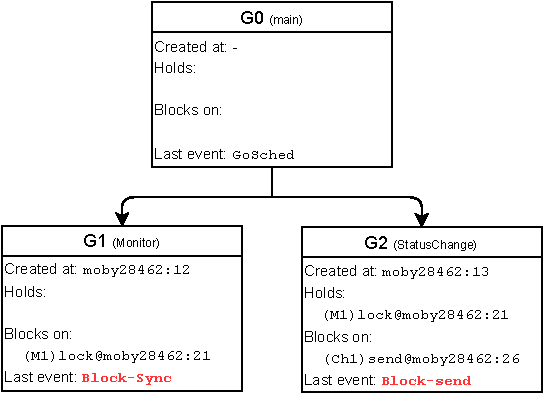
\includegraphics[width=0.75\linewidth]{figs/gtree.pdf}
%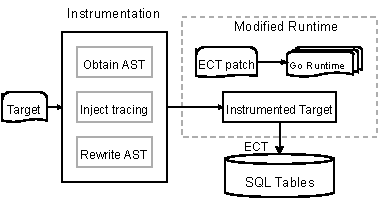
\includegraphics[]{figs/overview.png}
%\includegraphics[]{figs/overv}
\caption{Goroutine tree of the leaky interleaving in listing \ref{listing:moby28462}}
\label{fig:gtree}
\end{figure}

%
In addition to the parent/children relation of goroutines, nodes of the goroutine tree contains information about the goroutine creation site, the resources that it holds at each execution point and the final executed event right before program termination.
%
When tracing is enabled, every application goroutine invokes the tracer to capture $GoEnd$ before finishing its execution and exit (\ie change status from \textit{grunnable} to \textit{gdead}\cite{goexit-line-of-code}).
%
Before the main function returns, it calls the scheduler (through \texttt{runtime.Gosched()} invocation which captures $GoSched$ event) to hand over the control to the root goroutine to finish up program execution.
%
Since we instrument the application to call \texttt{runtime.traceStop} to stop tracing when main returns, $GoSched$ would be the last event captured for the main goroutine if it returns succesfully.
%

We call an execution \textbf{successful}, if below conditions hold
\begin{enumerate}
  \item (1) all goroutines spawned in the main goroutine has $GoEnd$ as their final event
  \item (2) the final event of the main goroutine is $GoSched$ with \texttt{runtime.traceStop} on top of its stack.
\end{enumerate}
If either of above conditions does not satisfy after program execution, a \textbf{deadlock} happens because it shows that there are one or more goroutines that did not reach its final state. \goat executes procedure \ref{proc:deadlockCheck} which is a BFS traversal on the goroutine tree to check if the program suffers from deadlocks.

\begin{small}
\begin{algorithm}[]
 \DontPrintSemicolon
 \SetKwFunction{KwDeadlockCheck}{DeadlockCheck}
% \SetKwInOut{Input}{Input} \SetKwInOut{Output}{Output}\SetKwInOut{Local}{Local}
  %\SetKw{KwEach}{each}
 %\Input{Stack of elements $S$, $S[1]$ is top}
 %\Output{$NLR(T)$}
 \KwDeadlockCheck{$G$}:{\\
 \Indp
    \If{$cur$.lastEvent$ \neq$ \texttt{GoSched}}{
      return \textbf{Global Deadlock}\;
    }
    $toVisit$ = $[G.children]$\;
    \For{ $|toVisit| \neq 0$}{
         $cur$ = $toVisit$[0]\;
         \If{$cur$.lastEvent $\neq$ \texttt{GoEnd}}{
            return \textbf{Partial Deadlock (leak)}\;
          }
         \For {$n$ in $cur.Children$}{
            append $n$ to $toVisit$\;
          }
          $toVisit = toVisit[1:]$\;
      }
      return \textbf{Pass}\;
  }
 \caption{\texttt{DeadlockCheck} procedure with root node of goroutine tree (main goroutine) as input}
 \label{proc:deadlockCheck}
\end{algorithm}
\end{small}



\subsubsection{Coverage Measurement}
Through a replay (\ie parsing the sequence) of ECT, a mapping between dynamic concurrent events and statically obtained CU points is emited by matching their respective call-stack and CU source location.
%
Through a BFS traversal of the goroutine tree, we add a \textit{coverage vector} to each goroutine node from the emitted mapping. Each element of the coverage vector is the respective covered value of requirement $R_i$ for the current goroutine node.
%
During executions of tests $t \in \mathcal{T}$, we maintain and update a global goroutine tree after each $t$.
%
It is crucial to maintain a global goroutine tree to measure the progress of coverage percentage over tests in $\mathcal{T}$.
%
Two goroutines $G_m$ and $G_n$ in the tests $t_i$ and $t_j$ are \textit{equivalent} (\ie falls into identical node in the global goroutine tree) if their parents are equivalent and their creation source location (CU of kind \texttt{go}) are identical:
\begin{equation}
  G_m \equiv G_n   \text{if}
  \begin{cases}
    \text{parent}(G_m) \equiv \text{parent}(G_n)  \wedge \\
    \text{CU(}G_m\text{).file} = \text{CU(}G_n\text{).file}  \wedge\\
    \text{CU(}G_m\text{).line} = \text{CU(}G_n\text{).line} \\
  \end{cases}
\end{equation}




\begin{table*}[]
\caption{Output of each debugging tool after experimenting on bug for GoKer \cite{yuan-gobench-cgo21} blocking bugs. For each tool, here is how to interprete its output: Detected bug (minimum \# of executions required) -- \textbf{X (1000)} means that the tool is not able to detect any bug after 1000 executions. \textbf{PDL}: Partial Deadlock, \textbf{GDL}: Global Deadlock, \textbf{PDL-k}: Partial Deadlock with \textit{k} number of goroutines leaked. \textbf{DL}: A warning for potential deadlock is issued. \textbf{TO/GDL}: The global deadlock is detected because none of goroutines made any progress after 20 seconds, \textbf{CRASH}: The execution paniced because of a flaw in the execution (e.g., send on closed channels panic), \textbf{HANG}: The tool halt for more than 10 minutes.}
\centering
\scalebox{0.75}{
    % Please add the following required packages to your document preamble:
% \usepackage{multirow}
% \usepackage[table,xcdraw]{xcolor}
% If you use beamer only pass "xcolor=table" option, i.e. \documentclass[xcolor=table]{beamer}
\begin{tabular}{|c|c|c|ccc|ccccc|}
\hline
\multicolumn{3}{|c|}{Bug Description} & \multicolumn{8}{c|}{Debugging Tools} \\ \hline
 &  &  & \multicolumn{1}{c|}{} & \multicolumn{1}{c|}{} &  & \multicolumn{5}{c|}{GOAT} \\ \cline{7-11}
\multirow{-2}{*}{Cause} & \multirow{-2}{*}{SubCause} & \multirow{-2}{*}{Bug ID} & \multicolumn{1}{c|}{\multirow{-2}{*}{BUILTINDL}} & \multicolumn{1}{c|}{\multirow{-2}{*}{GOLEAK}} & \multirow{-2}{*}{LOCKDL} & \multicolumn{1}{c|}{D0} & \multicolumn{1}{c|}{D1} & \multicolumn{1}{c|}{D2} & \multicolumn{1}{c|}{D3} & D4 \\ \hline
 &  & cockroach\_2448 & X (1000) & X (1000) & X (1000) & CRASH (1) & CRASH (1) & CRASH (1) & CRASH (1) & CRASH (1) \\ \cline{3-3}
 &  & cockroach\_24808 & GDL (1) & GDL (1) & TO/GDL (1) & TO/GDL (1) & TO/GDL (1) & TO/GDL (1) & TO/GDL (1) & TO/GDL (1) \\ \cline{3-3}
 &  & cockroach\_25456 & GDL (1) & GDL(1) & TO/GDL (1) & TO/GDL (1) & TO/GDL (1) & TO/GDL (1) & TO/GDL (1) & TO/GDL (1) \\ \cline{3-3}
 &  & cockroach\_35073 & GDL (1) & GDL (1) & TO/GDL (1) & TO/GDL (1) & TO/GDL (1) & TO/GDL (1) & TO/GDL (1) & TO/GDL (1) \\ \cline{3-3}
 &  & cockroach\_35931 & GDL (1) & GDL (1) & TO/GDL (1) & TO/GDL (1) & TO/GDL (1) & TO/GDL (1) & TO/GDL (1) & TO/GDL (1) \\ \cline{3-3}
 &  & etcd\_6857 & X (1000) & PDL (325) & X (1000) & \cellcolor[HTML]{EFEFEF}PDL-1 (1) & \cellcolor[HTML]{EFEFEF}PDL-1 (1) & \cellcolor[HTML]{EFEFEF}PDL-1 (11) & \cellcolor[HTML]{EFEFEF}PDL-1 (3) & \cellcolor[HTML]{EFEFEF}PDL-1 (3) \\ \cline{3-3}
 &  & grpc\_1275 & X (1000) & PDL (1) & X (1000) & PDL-1 (1) & PDL-1 (1) & PDL-1 (1) & PDL-1 (1) & PDL-1 (1) \\ \cline{3-3}
 &  & grpc\_1424 & X (1000) & PDL (1) & X (1000) & PDL-1 (1) & PDL-1 (1) & PDL-1 (1) & PDL-1 (1) & PDL-1 (1) \\ \cline{3-3}
 &  & grpc\_660 & X (1000) & PDL (1) & X (1000) & PDL-1 (1) & PDL-1 (1) & PDL-1 (1) & PDL-1 (1) & PDL-1 (1) \\ \cline{3-3}
 &  & istio\_17860 & X (1000) & PDL (1) & X (1000) & PDL-1 (2) & PDL-1 (1) & PDL-1 (1) & PDL-1 (1) & PDL-1 (1) \\ \cline{3-3}
 &  & kubernetes\_38669 & X (1000) & PDL (1) & X (1000) & PDL-1 (1) & PDL-1 (1) & PDL-1 (1) & PDL-1 (1) & PDL-1 (1) \\ \cline{3-3}
 &  & kubernetes\_5316 & X (1000) & PDL (1) & X (1000) & PDL-1 (1) & PDL-2 (1) & PDL-1 (1) & PDL-2 (1) & PDL-2 (1) \\ \cline{3-3}
 &  & kubernetes\_70277 & GDL (1) & GDL (1) & TO/GDL (1) & TO/GDL (1) & TO/GDL (1) & TO/GDL (1) & TO/GDL (1) & TO/GDL (1) \\ \cline{3-3}
 &  & moby\_21233 & X (1000) & PDL (1) & X (1000) & PDL-2 (1) & PDL-2 (1) & PDL-2 (1) & PDL-2 (1) & PDL-2 (1) \\ \cline{3-3}
 &  & moby\_33293 & X (1000) & PDL (1) & X (1000) & PDL-1 (1) & PDL-1 (3) & PDL-1 (1) & PDL-1 (1) & PDL-1 (1) \\ \cline{3-3}
 &  & moby\_4395 & X (1000) & PDL (1) & X (1000) & PDL-1 (1) & PDL-1 (1) & PDL-1 (1) & PDL-1 (1) & PDL-1 (1) \\ \cline{3-3}
 & \multirow{-17}{*}{Channel} & syncthing\_5795 & GDL (1) & GDL (1) & TO/GDL (1) & TO/GDL (1) & TO/GDL (1) & TO/GDL (1) & TO/GDL (1) & TO/GDL (1) \\ \cline{2-11}
 &  & kubernetes\_11298 & X (1000) & X (1000) & TO/GDL (179) & X (1000) & TO/GDL (352) & TO/GDL (158) & TO/GDL (179) & TO/GDL (179) \\ \cline{3-3}
 & \multirow{-2}{*}{\begin{tabular}[c]{@{}c@{}}Channel   \&\\      Conditional Variable\end{tabular}} & moby\_27782 & X (1000) & PDL (741) & X (1000) & X (1000) & \cellcolor[HTML]{EFEFEF}PDL-2 (1) & \cellcolor[HTML]{EFEFEF}PDL-2 (1) & \cellcolor[HTML]{EFEFEF}PDL-2 (4) & \cellcolor[HTML]{EFEFEF}PDL-2 (4) \\ \cline{2-11}
 &  & cockroach\_10790 & X (1000) & PDL (3) & X (1000) & PDL-2 (1) & PDL-2 (1) & PDL-2 (1) & PDL-2 (1) & PDL-2 (1) \\ \cline{3-3}
 &  & cockroach\_13197 & X (1000) & PDL (1) & X (1000) & PDL-1 (1) & PDL-1 (1) & PDL-1 (1) & PDL-1 (1) & PDL-1 (1) \\ \cline{3-3}
 &  & cockroach\_13755 & X (1000) & PDL (1) & X (1000) & PDL-1 (1) & PDL-1 (1) & PDL-1 (1) & PDL-1 (1) & PDL-1 (1) \\ \cline{3-3}
 &  & cockroach\_18101 & X (1000) & PDL (1) & X (1000) & PDL-1 (1) & PDL-1 (1) & PDL-1 (1) & PDL-1 (1) & PDL-1 (1) \\ \cline{3-3}
 &  & grpc\_862 & X (1000) & PDL (1) & X (1000) & PDL-1 (1) & PDL-1 (1) & PDL-1 (1) & PDL-1 (1) & PDL-1 (1) \\ \cline{3-3}
 &  & istio\_18454 & X (1000) & PDL (13) & X (1000) & PDL-2 (5) & PDL-1 (14) & PDL-1 (4) & PDL-1 (6) & PDL-1 (6) \\ \cline{3-3}
 &  & kubernetes\_25331 & X (1000) & PDL (1) & X (1000) & PDL-1 (1) & PDL-1 (1) & PDL-1 (1) & PDL-1 (1) & PDL-1 (1) \\ \cline{3-3}
 & \multirow{-8}{*}{\begin{tabular}[c]{@{}c@{}}Channel \& \\      Context\end{tabular}} & moby\_33781 & X (1000) & PDL (1) & X (1000) & PDL-1 (221) & PDL-1 (10) & PDL-1 (8) & PDL-1 (10) & PDL-1 (10) \\ \cline{2-11}
 &  & moby\_29733 & GDL (1) & GDL (1) & TO/GDL (1) & TO/GDL (1) & TO/GDL (1) & TO/GDL (1) & TO/GDL (1) & TO/GDL (1) \\ \cline{3-3}
\multirow{-29}{*}{\begin{tabular}[c]{@{}c@{}}Communication\\       Deadlock\end{tabular}} & \multirow{-2}{*}{Condition Variable} & moby\_30408 & GDL (1) & GDL (1) & TO/GDL (1) & TO/GDL (1) & TO/GDL (1) & TO/GDL (1) & TO/GDL (1) & TO/GDL (1) \\ \hline
 &  & etcd\_6873 & X (1000) & PDL (371) & X (1000) & PDL-2 (1) & PDL-2 (2) & PDL-2 (7) & PDL-2 (6) & PDL-2 (6) \\ \cline{3-3}
 &  & etcd\_7443 & X (1000) & X (1000) & X (1000) & X (1000) & \cellcolor[HTML]{EFEFEF}PDL-1 (9) & \cellcolor[HTML]{EFEFEF}PDL-1 (15) & \cellcolor[HTML]{EFEFEF}PDL-1 (14) & \cellcolor[HTML]{EFEFEF}PDL-1 (14) \\ \cline{3-3}
 &  & etcd\_7492 & HANG (1) & HANG (1) & TO/GDL (4) & TO/GDL (1) & TO/GDL (1) & TO/GDL (1) & TO/GDL (1) & TO/GDL (1) \\ \cline{3-3}
 &  & etcd\_7902 & X (1000) & PDL (1) & X (1000) & PDL-4 (1) & PDL-4 (1) & PDL-4 (1) & PDL-4 (1) & PDL-4 (1) \\ \cline{3-3}
 &  & grpc\_1353 & X (1000) & PDL (1) & X (1000) & CRASH (1) & CRASH (1) & PDL-3 (1) & PDL-3 (1) & PDL-3 (1) \\ \cline{3-3}
 &  & grpc\_1460 & X (1000) & PDL (1) & X (1000) & PDL-2 (135) & PDL-2 (1) & PDL-2 (2) & PDL-2 (1) & PDL-2 (1) \\ \cline{3-3}
 &  & istio\_16224 & GDL (1) & GDL (1) & TO/GDL (1) & TO/GDL (1) & TO/GDL (1) & TO/GDL (1) & TO/GDL (1) & TO/GDL (1) \\ \cline{3-3}
 &  & kubernetes\_10182 & X (1000) & PDL (44) & X (1000) & \cellcolor[HTML]{EFEFEF}PDL-2 (1) & \cellcolor[HTML]{EFEFEF}PDL-2 (1) & \cellcolor[HTML]{EFEFEF}PDL-2 (1) & \cellcolor[HTML]{EFEFEF}PDL-2 (1) & \cellcolor[HTML]{EFEFEF}PDL-2 (1) \\ \cline{3-3}
 &  & kubernetes\_1321 & X (1000) & PDL (307) & X (1000) & X (1000) & \cellcolor[HTML]{EFEFEF}PDL-1 (1) & \cellcolor[HTML]{EFEFEF}PDL-1 (1) & \cellcolor[HTML]{EFEFEF}PDL-1 (1) & \cellcolor[HTML]{EFEFEF}PDL-1 (1) \\ \cline{3-3}
 &  & kubernetes\_26980 & GDL (375) & GDL (131) & X (1000) & TO/GDL (191) & TO/GDL (1) & TO/GDL (1) & TO/GDL (1) & TO/GDL (1) \\ \cline{3-3}
 &  & kubernetes\_6632 & X (1000) & X (1000) & X (1000) & \cellcolor[HTML]{EFEFEF}PDL-2 (1) & \cellcolor[HTML]{EFEFEF}PDL-2 (1) & \cellcolor[HTML]{EFEFEF}PDL-2 (2) & \cellcolor[HTML]{EFEFEF}PDL-2 (1) & \cellcolor[HTML]{EFEFEF}PDL-2 (1) \\ \cline{3-3}
 &  & moby\_28462 & X (1000) & PDL (5) & X (1000) & PDL-2 (39) & PDL-2 (1) & PDL-2 (1) & PDL-2 (1) & PDL-2 (1) \\ \cline{3-3}
 & \multirow{-13}{*}{Channel \& Lock} & serving\_2137 & X (1000) & X (1000) & X (1000) & X (1000) & X (1000) & TO/GDL (88) & X (1000) & X (1000) \\ \cline{2-11}
 &  & cockroach\_1055 & GDL (1) & GDL (1) & TO/GDL (1) & TO/GDL (1) & TO/GDL (1) & TO/GDL (1) & TO/GDL (1) & TO/GDL (1) \\ \cline{3-3}
 & \multirow{-2}{*}{\begin{tabular}[c]{@{}c@{}}Channel   \& \\      WaitGroup\end{tabular}} & cockroach\_1462 & X (1000) & X (1000) & TO/GDL (1) & X (1000) & TO/GDL (1) & TO/GDL (1) & TO/GDL (1) & TO/GDL (1) \\ \cline{2-11}
\multirow{-16}{*}{\begin{tabular}[c]{@{}c@{}}Mixed \\      Deadlock\end{tabular}} & Misuse WaitGroup & moby\_25384 & X (1000) & PDL (1) & X (1000) & PDL-1 (1) & PDL-1 (1) & PDL-1 (1) & PDL-1 (1) & PDL-1 (1) \\ \hline
 &  & cockroach\_584 & X (1000) & PDL (1) & X (1000) & PDL-1 (1) & PDL-1 (1) & PDL-1 (1) & PDL-1 (1) & PDL-1 (1) \\ \cline{3-3}
 &  & cockroach\_9935 & X (1000) & PDL (1) & DL (721) & PDL-1 (1) & PDL-1 (2) & PDL-1 (1) & PDL-1 (1) & PDL-1 (1) \\ \cline{3-3}
 &  & etcd\_10492 & GDL (1) & GDL (1) & DL (1) & TO/GDL (1) & TO/GDL (1) & TO/GDL (1) & TO/GDL (1) & TO/GDL (1) \\ \cline{3-3}
 &  & etcd\_5509 & X (1000) & GDL (766) & TO/GDL (426) & X (1000) & TO/GDL (1) & TO/GDL (1) & TO/GDL (1) & TO/GDL (1) \\ \cline{3-3}
 &  & etcd\_6708 & GDL (1) & GDL (1) & DL (1) & TO/GDL (1) & TO/GDL (1) & TO/GDL (1) & TO/GDL (1) & TO/GDL (1) \\ \cline{3-3}
 &  & grpc\_3017 & GDL (4) & GDL (4) & TO/GDL (3) & TO/GDL (1) & TO/GDL (1) & TO/GDL (1) & TO/GDL (1) & TO/GDL (1) \\ \cline{3-3}
 &  & grpc\_795 & GDL (1) & GDL (1) & DL (1) & TO/GDL (1) & TO/GDL (1) & TO/GDL (1) & TO/GDL (1) & TO/GDL (1) \\ \cline{3-3}
 &  & hugo\_5379 & GDL (1) & GDL (1) & TO/GDL (1) & TO/GDL (1) & TO/GDL (1) & TO/GDL (1) & TO/GDL (1) & TO/GDL (1) \\ \cline{3-3}
 &  & moby\_17176 & X (1000) & PDL (1) & X (1000) & PDL-1 (1) & PDL-1 (1) & PDL-1 (1) & PDL-1 (1) & PDL-1 (1) \\ \cline{3-3}
 &  & moby\_36114 & X (1000) & PDL (1) & X (1000) & PDL-1 (1) & PDL-1 (1) & PDL-1 (1) & PDL-1 (1) & PDL-1 (1) \\ \cline{3-3}
 &  & moby\_7559 & X (1000) & PDL (1) & X (1000) & PDL-1 (1) & PDL-1 (1) & PDL-1 (1) & PDL-1 (1) & PDL-1 (1) \\ \cline{3-3}
 & \multirow{-12}{*}{Double locking} & syncthing\_4829 & GDL (1) & GDL (1) & DL (1) & TO/GDL (1) & TO/GDL (1) & TO/GDL (1) & TO/GDL (1) & TO/GDL (1) \\ \cline{2-11}
 &  & cockroach\_16167 & X (1000) & X (1000) & DL (1) & X (1000) & TO/GDL (1) & TO/GDL (1) & TO/GDL (1) & TO/GDL (1) \\ \cline{3-3}
 &  & cockroach\_3710 & X (1000) & X (1000) & DL (123) & \cellcolor[HTML]{EFEFEF}PDL-2 (28) & \cellcolor[HTML]{EFEFEF}PDL-2 (1) & \cellcolor[HTML]{EFEFEF}PDL-2 (1) & \cellcolor[HTML]{EFEFEF}PDL-2 (1) & \cellcolor[HTML]{EFEFEF}PDL-2 (1) \\ \cline{3-3}
 &  & cockroach\_6181 & X (1000) & PDL (1) & X (1000) & PDL-4 (1) & PDL-4 (1) & PDL-3 (1) & PDL-1 (1) & PDL-1 (1) \\ \cline{3-3}
 &  & hugo\_3251 & GDL (1) & GDL (1) & DL (1) & TO/GDL (1) & TO/GDL (1) & TO/GDL (1) & TO/GDL (1) & TO/GDL (1) \\ \cline{3-3}
 &  & kubernetes\_58107 & X (1000) & X (1000) & X (1000) & \cellcolor[HTML]{EFEFEF}PDL-1 (1) & \cellcolor[HTML]{EFEFEF}PDL-1 (1) & \cellcolor[HTML]{EFEFEF}PDL-1 (1) & \cellcolor[HTML]{EFEFEF}PDL-1 (1) & \cellcolor[HTML]{EFEFEF}PDL-1 (1) \\ \cline{3-3}
 & \multirow{-6}{*}{RWR deadlock} & kubernetes\_62464 & X (1000) & X (1000) & DL (6) & PDL-2 (161) & PDL-2 (7) & PDL-2 (2) & PDL-2 (3) & PDL-2 (3) \\ \cline{2-11}
 &  & cockroach\_10214 & X (1000) & X (1000) & X (1000) & \cellcolor[HTML]{EFEFEF}PDL-2 (368) & \cellcolor[HTML]{EFEFEF}PDL-2 (1) & \cellcolor[HTML]{EFEFEF}PDL-2 (1) & \cellcolor[HTML]{EFEFEF}PDL-2 (1) & \cellcolor[HTML]{EFEFEF}PDL-2 (1) \\ \cline{3-3}
 &  & cockroach\_7504 & X (1000) & X (1000) & X (1000) & \cellcolor[HTML]{EFEFEF}PDL-2 (199) & \cellcolor[HTML]{EFEFEF}PDL-2 (1) & \cellcolor[HTML]{EFEFEF}PDL-2 (7) & \cellcolor[HTML]{EFEFEF}PDL-2 (1) & \cellcolor[HTML]{EFEFEF}PDL-2 (1) \\ \cline{3-3}
 &  & kubernetes\_13135 & X (1000) & PDL (1) & DL (4) & PDL-2 (1) & PDL-2 (5) & PDL-2 (1) & PDL-2 (22) & PDL-2 (22) \\ \cline{3-3}
 &  & kubernetes\_30872 & X (1000) & PDL (338) & X (1000) & \cellcolor[HTML]{EFEFEF}PDL-3 (50) & \cellcolor[HTML]{EFEFEF}PDL-3 (2) & \cellcolor[HTML]{EFEFEF}PDL-3 (1) & \cellcolor[HTML]{EFEFEF}PDL-3 (6) & \cellcolor[HTML]{EFEFEF}PDL-3 (6) \\ \cline{3-3}
\multirow{-23}{*}{\begin{tabular}[c]{@{}c@{}}Resource \\      Deadlock\end{tabular}} & \multirow{-5}{*}{AB-BA deadlock} & moby\_4951 & X (1000) & PDL (120) & X (1000) & \cellcolor[HTML]{EFEFEF}PDL-2 (15) & \cellcolor[HTML]{EFEFEF}PDL-2 (2) & \cellcolor[HTML]{EFEFEF}PDL-2 (2) & \cellcolor[HTML]{EFEFEF}PDL-2 (1) & \cellcolor[HTML]{EFEFEF}PDL-2 (1) \\ \hline
\multicolumn{1}{|l|}{Total Bugs:} & \multicolumn{1}{l|}{68} & \multicolumn{1}{l|}{Total Detected:} & 19 & 56 & 26 & 60 & 67 & 68 & 67 & 67 \\ \hline
\end{tabular}

  }
\label{tab:comparison}
\end{table*}




\subsection{Instrumentation}
\label{sec:dl_instrument}



\begin{table}[]
\centering
\caption{Concurrency Usages and coverage requirements of program in listing\ref{listing:moby28462.minipage}}
\scalebox{0.9}{

\begin{tabular}{
>{\columncolor[HTML]{FFFFFF}}c
>{\columncolor[HTML]{FFFFFF}}l |
>{\columncolor[HTML]{FFFFFF}}l |
>{\columncolor[HTML]{FFFFFF}}c |
>{\columncolor[HTML]{FFFFFF}}c |
>{\columncolor[HTML]{FFFFFF}}c |}
\hline
\multicolumn{2}{|c|}{\cellcolor[HTML]{FFFFFF}CU of list. \ref{listing:moby28462.minipage}} & \multicolumn{1}{c|}{\cellcolor[HTML]{FFFFFF}} & \multicolumn{2}{c|}{\cellcolor[HTML]{FFFFFF}Covered by} & \cellcolor[HTML]{FFFFFF} \\ \cline{1-2} \cline{4-5}
\multicolumn{1}{|c|}{\cellcolor[HTML]{FFFFFF}Line} & \multicolumn{1}{c|}{\cellcolor[HTML]{FFFFFF}Kind} & \multicolumn{1}{c|}{\multirow{-2}{*}{\cellcolor[HTML]{FFFFFF}Coverage Requirements}} & run \#1 & run \#2 & \multirow{-2}{*}{\cellcolor[HTML]{FFFFFF}\begin{tabular}[c]{@{}c@{}}Overall\\      Covered\end{tabular}} \\ \hline
\multicolumn{1}{|c|}{\cellcolor[HTML]{FFFFFF}12} & go & covered & $\checkmark_{G0}$ & $\checkmark_{G0}$ & $\checkmark$ \\ \hline
\multicolumn{1}{|c|}{\cellcolor[HTML]{FFFFFF}13} & go & covered & $\checkmark_{G0}$ & $\checkmark_{G0}$ & $\checkmark$ \\ \hline
\multicolumn{1}{|c|}{\cellcolor[HTML]{FFFFFF}} & \cellcolor[HTML]{FFFFFF} & c-recv-blocked & $\checkmark_{G1}$ &  & $\checkmark$ \\ \cline{3-6}
\multicolumn{1}{|c|}{\multirow{-2}{*}{\cellcolor[HTML]{FFFFFF}17}} & \multirow{-2}{*}{\cellcolor[HTML]{FFFFFF}select} & c-recv-unblocking & $\checkmark_{G1}$ &  & $\checkmark$ \\ \hline
\multicolumn{1}{|c|}{\cellcolor[HTML]{FFFFFF}} & \cellcolor[HTML]{FFFFFF} & blocked &  & \cellcolor[HTML]{C0C0C0}$\checkmark_{G1}$ & $\checkmark$ \\ \cline{3-6}
\multicolumn{1}{|c|}{\multirow{-2}{*}{\cellcolor[HTML]{FFFFFF}21}} & \multirow{-2}{*}{\cellcolor[HTML]{FFFFFF}lock} & blocking & $\checkmark_{G1}$ &  & $\checkmark$ \\ \hline
\multicolumn{1}{|c|}{\cellcolor[HTML]{FFFFFF}} & \cellcolor[HTML]{FFFFFF} & unblocking & $\checkmark_{G1}$ &  & $\checkmark$ \\ \cline{3-6}
\multicolumn{1}{|c|}{\multirow{-2}{*}{\cellcolor[HTML]{FFFFFF}22}} & \multirow{-2}{*}{\cellcolor[HTML]{FFFFFF}unlock} & no\_op &  &  &  \\ \hline
\multicolumn{1}{|c|}{\cellcolor[HTML]{FFFFFF}} & \cellcolor[HTML]{FFFFFF} & blocked & $\checkmark_{G2}$ &  & $\checkmark$ \\ \cline{3-6}
\multicolumn{1}{|c|}{\multirow{-2}{*}{\cellcolor[HTML]{FFFFFF}25}} & \multirow{-2}{*}{\cellcolor[HTML]{FFFFFF}lock} & blocking &  & \cellcolor[HTML]{C0C0C0} \textbf{$\checkmark_{G2}$} & $\checkmark$ \\ \hline
\multicolumn{1}{|c|}{\cellcolor[HTML]{FFFFFF}} & \cellcolor[HTML]{FFFFFF} & blocked & $\checkmark_{G2}$ & $\checkmark_{G2}$ & $\checkmark$ \\ \cline{3-6}
\multicolumn{1}{|c|}{\cellcolor[HTML]{FFFFFF}} & \cellcolor[HTML]{FFFFFF} & unblocking &  &  &  \\ \cline{3-6}
\multicolumn{1}{|c|}{\multirow{-3}{*}{\cellcolor[HTML]{FFFFFF}26}} & \multirow{-3}{*}{\cellcolor[HTML]{FFFFFF}send} & no\_op &  &  &  \\ \hline
\multicolumn{1}{|c|}{\cellcolor[HTML]{FFFFFF}} & \cellcolor[HTML]{FFFFFF} & unblocking &  &  &  \\ \cline{3-6}
\multicolumn{1}{|c|}{\multirow{-2}{*}{\cellcolor[HTML]{FFFFFF}27}} & \multirow{-2}{*}{\cellcolor[HTML]{FFFFFF}unlock} & no\_op & $\checkmark_{G2}$ &  & $\checkmark$ \\ \hline
\multicolumn{1}{l}{\cellcolor[HTML]{FFFFFF}} &  & Coverage \% & 60\% & 33\% & 73\% \\ \cline{3-6}
\end{tabular}

}
\label{tab:moby_cov_table}
\end{table}
